% !TeX encoding = UTF-8
\chapter{\iftoggle{lang_eng}{Appendix}{Anhang}}
\label{app:Anhang1}


\begin{table}[H]
    \centering
    \resizebox{\textwidth}{!}{%
    \begin{tabular}{|l|l|l|}
    \hline
    \textbf{Feature Category} & \textbf{Feature} & \textbf{Description} \\ \hline
    \multirow{8}{*}{Statistical Features} & eda\_mean & Mean of EDA signal \\ 
     & eda\_std & Standard deviation of EDA signal \\ 
     & eda\_max & Maximum value of EDA signal \\
     & eda\_min & Minimum value of EDA signal \\
     & eda\_range & Range of EDA signal (max - min) \\
     & eda\_kurtosis & Kurtosis of EDA signal \\
     & eda\_skew & Skewness of EDA signal \\
     & eda\_momentum & Overall momentum of EDA signal \\ \hline
    \multirow{5}{*}{Frequency-Domain Features} & eda\_f1sc, eda\_f2sc, eda\_f3sc & Frequency-specific components \\
     & eda\_Energy & Total energy of EDA signal \\
     & eda\_Entropy & Entropy of EDA signal \\
     & eda\_max\_freq & Maximum frequency in EDA signal \\ \hline
    \multirow{15}{*}{SCR Features} & scr\_mean & Mean of SCR signal \\
     & scr\_std & Standard deviation of SCR signal \\
     & scr\_max, scr\_min, scr\_range & Various measures of SCR \\
     & scr\_kurtosis, scr\_skew & Kurtosis and Skewness of SCR \\
     & scr\_momentum & Overall momentum of SCR signal \\
     & scr\_activity, scr\_complexity & Activity and complexity measures \\
     & scr\_mobility, scr\_rms & Mobility and RMS of SCR \\
     & scr\_acr\_length, scr\_integral & ACR length and integral of SCR \\
     & scr\_average\_power & Average power of SCR \\
     & scr\_f1sc, scr\_f2sc, scr\_f3sc & Frequency-specific components of SCR \\
     & scr\_Energy & Total energy of SCR signal \\
     & scr\_Entropy & Entropy of SCR signal \\
     & scr\_max\_freq & Maximum frequency in SCR signal \\ \hline
    \multirow{8}{*}{SCL Features} & scl\_mean, scl\_std & Mean and Standard deviation of SCL \\
     & scl\_max, scl\_min & Maximum and Minimum value of SCL \\
     & scl\_range & Range of SCL \\
     & scl\_kurtosis, scl\_skew & Kurtosis and Skewness of SCL \\
     & scl\_momentum & Overall momentum of SCL \\ \hline
    \end{tabular}
    }
    \caption{EDA Features Overview}
    \label{tab:eda_features}
    \end{table}
    
    \begin{table}[H]
        \centering
        \resizebox{\textwidth}{!}{%
        \begin{tabular}{|l|l|l|}
        \hline
        \textbf{Parameter Type} & \textbf{Feature} & \textbf{Description} \\ \hline
        \multirow{19}{*}{Time-domain HRV} & mean\_nni & Mean of peak to peak intervals \\ 
         & sdnn & Standard deviation of peak to peak intervals \\ 
         & rmssd & Root mean square of successive differences \\
         & sdsd & Standard deviation of successive differences \\
         & nni\_50 & Number of pairs of intervals differing by more than 50 ms \\
         & pnni\_50 & Ratio of nni\_50 to total number of intervals \\
         & nni\_20 & Number of pairs of intervals differing by more than 20 ms \\
         & pnni\_20 & Ratio of nni\_20 to total number of intervals \\
         & cvnni & Ratio of sdnn to mean\_nni \\
         & cvsd & Ratio of rmssd to mean\_nni \\
         & median\_nni & Median of successive differences \\
         & range\_nni & Range of peak to peak intervals \\
         & mean\_hr & Mean heart rate \\
         & min\_hr & Minimum heart rate \\
         & max\_hr & Maximum heart rate \\
         & std\_hr & Standard deviation of heart rate \\
         & mad\_nni & Mean absolute deviation of intervals \\
         & mcv\_nni & Ratio of mead\_nni to median\_nni \\
         & iqr\_nni & Interquartile range of intervals \\ \hline
        \multirow{12}{*}{Frequency-domain HRV} & vlf & Very low frequency power \\
         & lf & Low frequency power \\
         & hf & High frequency power \\
         & lf\_hf\_ratio & Ratio of lf to hf \\
         & total\_power & Sum of vlf, lf, and hf \\
         & lfnu & Normalized lf power \\
         & hfnu & Normalized hf power \\
         & lnLF & Log transformed low-frequency power \\
         & lnHF & Log transformed high-frequency power \\
         & vlf\_peak & Max peak in very low frequency band \\
         & lf\_peak & Max peak in low frequency band \\
         & hf\_peak & Max peak in high frequency band \\ \hline
        \multirow{9}{*}{Nonlinear HRV} & SD1 & SD of Poincare plot perpendicular to identity line \\
         & SD2 & SD of Poincare plot along the identity line \\
         & SD2\_SD1 & Ratio of SD2 to SD1 \\
         & CSI & Cardiac stress index \\
         & CVI & Cardiac vagal index \\
         & CSI\_modified & Modified cardiac stress index \\
         & ApEn & Approximate entropy of intervals \\
         & SampEn & Sample entropy of intervals \\ \hline
        \end{tabular}
        }
        \caption{PPG-HRV Features Overview}
        \label{tab:ppg_hrv_features}
        \end{table}
        



\begin{figure}[!htbp]
	\centering
	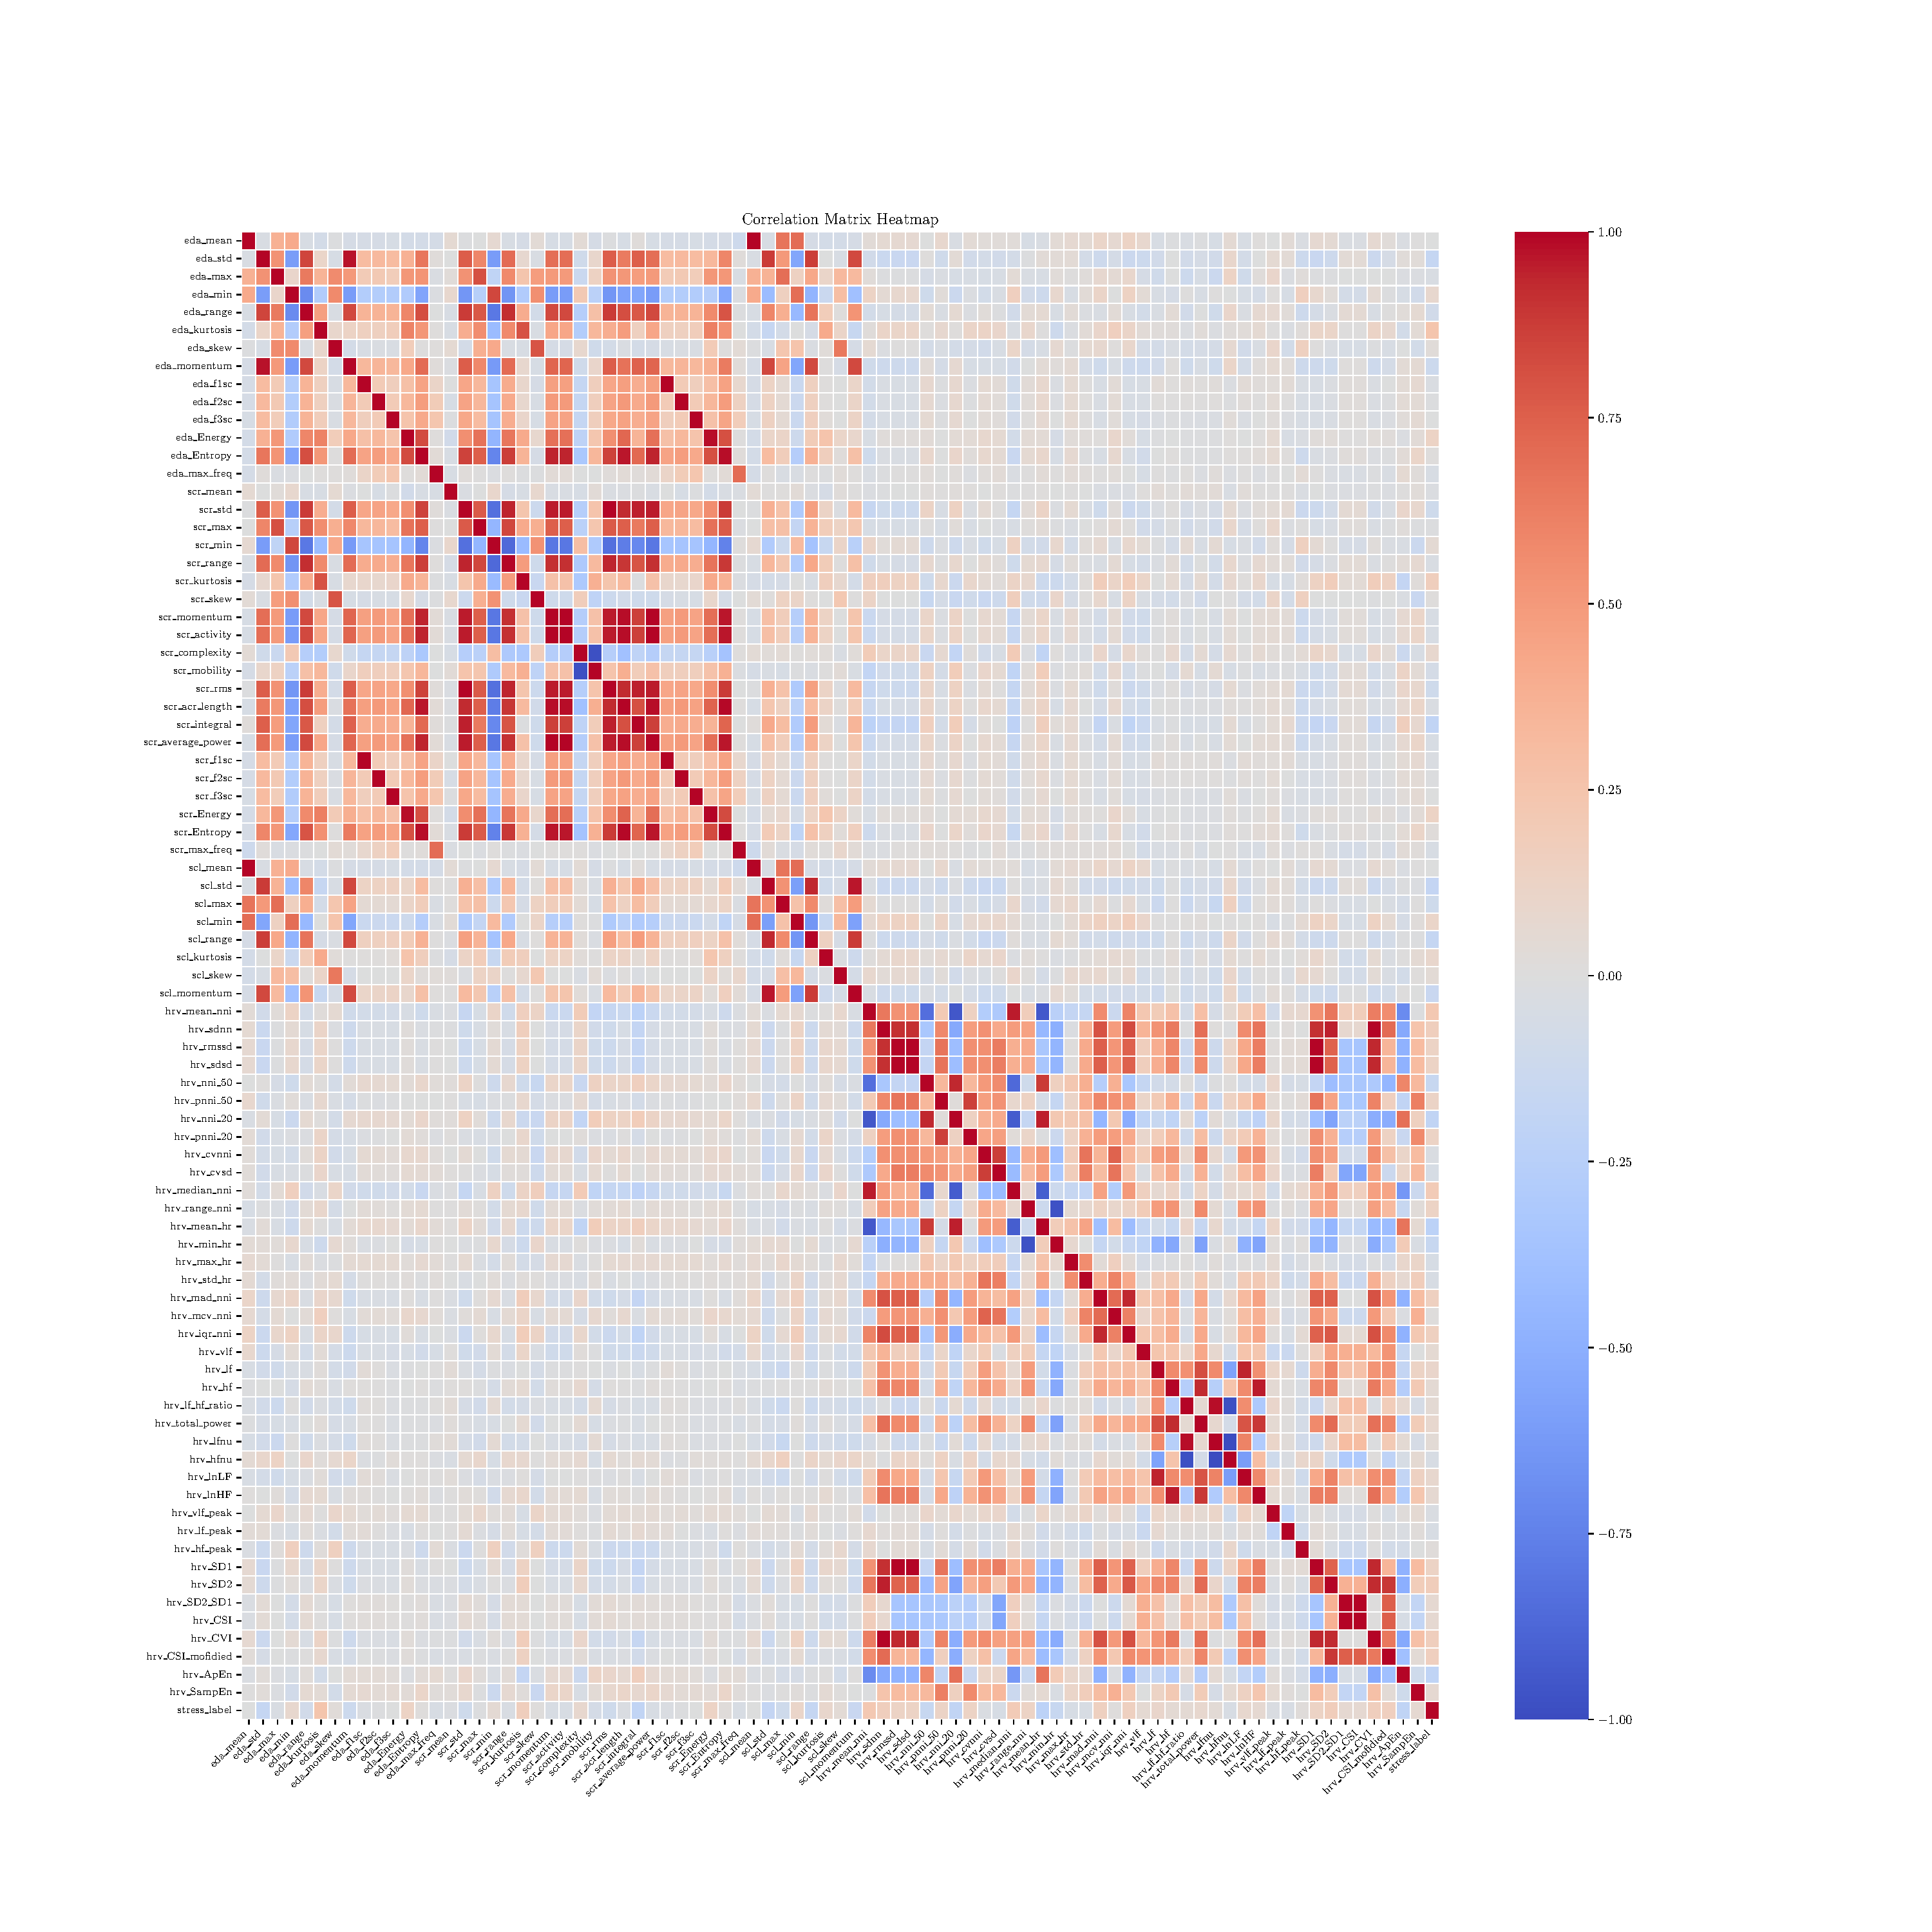
\includegraphics[width=\columnwidth]{images/correlation_matrix_heatmap.pdf}
	\caption{Correlation matrix for feature selection}
	\label{fig:netwrok}
\end{figure}



\newpage
\section{\iftoggle{lang_eng}{Usage of generative AI - Affidavit}{Erklärung zur Nutzung generativer KI-Modelle}}
\label{app:erklaerung}
\iftoggle{thesis_phd}{
    \begin{itemize}
        \item[$\square$] {\iftoggle{lang_eng}{not at all}{gar nicht}}
        \item[$\boxtimes$] {\iftoggle{lang_eng}{for correcting, optimizing, or restructuring the entire work (This eliminates the need for explicit marking of individual passages or sections, as this type of usage refers to the entire written work. Explicit marking in the text is not necessary, as this serves as the global indication.)}{zur Korrektur, Optimierung oder Umstrukturierung der gesamten Arbeit (Dies erübrigt eine explizite Markierung einzelner Passagen oder Abschnitte, da sich diese Art der Nutzung auf die gesamte schriftliche Ausarbeitung bezieht. Eine explizite Markierung im Text ist nicht notwendig, da hiermit die globale Kenntlichmachung erfolgt.)}}

        %Code
        \item[\ifglsused{gptco}{$\boxtimes$}{$\square$}] {\iftoggle{lang_eng}{Code optimization: Optimization or restructuring of software function}{Codeoptimierend: Optimierung oder Umstrukturierung von Software-Funktionen}}
        \item[\ifglsused{gptcg}{$\boxtimes$}{$\square$}] {\iftoggle{lang_eng}{Code generation: Creating entire software functions from a detailed functional description.}{Codegenerierend: Erstellung ganzer Software-Funktionen aus einer
        detailierten Funktionsbeschreibung}}
        \item[\ifglsused{gptcs}{$\boxtimes$}{$\square$}] {\iftoggle{lang_eng}{Substance generation in code: Generating entire software source code}{Code-Substanzgenerierend: Erzeugung ganzer Software-Quelltexte}}
        %Media
        \item[\ifglsused{gptmo}{$\boxtimes$}{$\square$}] {\iftoggle{lang_eng}{Media optimization: Correction, optimization, or restructuring of entire passages}{Medienoptimierend: Korrektur, Optimierung oder Umstrukturierung
        ganzer Passagen}}
        \item[\ifglsused{gptmg}{$\boxtimes$}{$\square$}] {\iftoggle{lang_eng}{Media generation: Creating entire passages from given content.}{Mediengenerierend: Erstellen ganzer Passagen aus vorgegebenem Inhalt}}
        \item[\ifglsused{gptms}{$\boxtimes$}{$\square$}] {\iftoggle{lang_eng}{Substance generation in media: Generating entire sections}{Medien-Substanzgenerierend: Erzeugung ganzer Abschnitte}}
        \item[\ifglsused{gptx}{$\boxtimes$}{$\square$}] {\iftoggle{lang_eng}{More, namely:}{Weiteres, nämlich:}}

    \end{itemize}
    \hrulefill

    \hrulefill

    \hrulefill

    \hrulefill

    {\iftoggle{lang_eng}{I assure that I have provided all usages completely. Missing or incorrect information may be considered an attempt to deceive.}{Ich versichere, alle Nutzungen vollständig angegeben zu haben. Fehlende oder fehlerhafte Angaben können als Täuschungsversuch gewertet werden.}}
    \\[10pt]
}
{
    \begin{itemize}
        \item[$\square$] {\iftoggle{lang_eng}{not at all}{gar nicht}}
        \item[$\boxtimes$] {\iftoggle{lang_eng}{for correcting, optimizing, or restructuring the entire work (This eliminates the need for explicit marking of individual passages or sections, as this type of usage refers to the entire written work. Explicit marking in the text is not necessary, as this serves as the global indication.)}{zur Korrektur, Optimierung oder Umstrukturierung der gesamten Arbeit (Dies erübrigt eine explizite Markierung einzelner Passagen oder Abschnitte, da sich diese Art der Nutzung auf die gesamte schriftliche Ausarbeitung bezieht. Eine explizite Markierung im Text ist nicht notwendig, da hiermit die globale Kenntlichmachung erfolgt.)}}

        %Code
        \item[$\boxtimes$] {\iftoggle{lang_eng}{Code optimization: Optimization or restructuring of software function}{Codeoptimierend: Optimierung oder Umstrukturierung von Software-Funktionen}}
        \item[$\boxtimes$] {\iftoggle{lang_eng}{Code generation: Creating entire software functions from a detailed functional description.}{Codegenerierend: Erstellung ganzer Software-Funktionen aus einer
        detailierten Funktionsbeschreibung}}
        \item[$\square$] {\iftoggle{lang_eng}{Substance generation in code: Generating entire software source code}{Code-Substanzgenerierend: Erzeugung ganzer Software-Quelltexte}}
        %Media
        \item[$\boxtimes$] {\iftoggle{lang_eng}{Media optimization: Correction, optimization, or restructuring of entire passages}{Medienoptimierend: Korrektur, Optimierung oder Umstrukturierung
        ganzer Passagen}}
        \item[$\boxtimes$] {\iftoggle{lang_eng}{Media generation: Creating entire passages from given content.}{Mediengenerierend: Erstellen ganzer Passagen aus vorgegebenem Inhalt}}
        \item[$\square$] {\iftoggle{lang_eng}{Substance generation in media: Generating entire sections}{Medien-Substanzgenerierend: Erzeugung ganzer Abschnitte}}
        \item[$\square$] {\iftoggle{lang_eng}{More, namely:}{Weiteres, nämlich:}}

    \end{itemize}
    \hrulefill

    \hrulefill

    \hrulefill

    \hrulefill

    {\iftoggle{lang_eng}{I assure that I have provided all usages completely. Missing or incorrect information may be considered an attempt to deceive.}{Ich versichere, alle Nutzungen vollständig angegeben zu haben. Fehlende oder fehlerhafte Angaben können als Täuschungsversuch gewertet werden.}}
    \\[10pt]
}
% {
% \begin{itemize}
%     \item[$\square$] gar nicht
%     \item[$\boxtimes$] zur Korrektur, Optimierung oder Umstrukturierung der gesamten Arbeit (Dies erübrigt eine explizite Markierung einzelner Passagen oder Abschnitte, da sich diese Art der Nutzung auf die gesamte schriftliche Ausarbeitung bezieht. Eine explizite Markierung im Text ist nicht notwendig, da hiermit die globale Kenntlichmachung erfolgt.)
%     \item[\ifglsused{gptie}{$\boxtimes$}{$\square$}] zum Erzeugen ganzer Abschnitte (inhaltserzeugend)
%     \item[\ifglsused{gptte}{$\boxtimes$}{$\square$}] zum Erstellen ganzer Passagen aus vorgegebenem Inhalt (texterzeugend)
%     \item[\ifglsused{gpt}{$\boxtimes$}{$\square$}] zur Korrektur, Optimierung oder Umstrukturierung ganzer Passagen (textoptimierend)

%     \item[\ifglsused{gptme}{$\boxtimes$}{$\square$}] zum Erzeugen ganzer Software-Quelltexte (mehrwerterzeugend)
%     \item[\ifglsused{gptce}{$\boxtimes$}{$\square$}] zum Erstellen ganzer Software-Funktionen aus einer detailierten Funktionsbeschreibung (codeerzeugend)
%     \item[\ifglsused{gptco}{$\boxtimes$}{$\square$}] zur Optimierung oder Umstrukturierung von Software-Funktionen (codeoptimierend)
%     \item[\ifglsused{gptx}{$\boxtimes$}{$\square$}] Weiteres, nämlich:
% \end{itemize}
% \hrulefill

% \hrulefill

% \hrulefill

% \hrulefill

% 
% \\[10pt]
% }
%\parbox{4cm}{\hrule
%\strut \centering\footnotesize \iftoggle{lang_eng}{Dortmund, 21.02.2024}{Ort, Datum}} \hfill\parbox{4cm}{\hrule
%\strut \centering\footnotesize Mohammed Faizan}

\parbox{4cm}{
    \strut \centering\footnotesize \iftoggle{lang_eng}{Dortmund, 21.02.2024}{Ort, Datum}
} \hfill
\parbox{4cm}{
    \strut \centering\footnotesize Mohammed Faizan
}